\documentclass[compress, darktitle, framenumber, totalframenumber]{beamer}
\usepackage{booktabs}
\usepackage{mathtools}
\usepackage{tikz}
\usepackage{wasysym}
\usepackage{wrapfig}
\usepackage{xparse}

\mathtoolsset{showonlyrefs}

\usetheme{UniversiteitAntwerpen}

\title{Wisku$\mathbb{N}$de in-$\mathbb{Z}$icht}
\subtitle{Wiskunde in muziek}
\author{Pieter Belmans (\texttt{pieter.belmans@uantwerpen.be}) \\ Matthias Roels (\texttt{matthias.roels@uantwerpen.be})}
\date{9 januari 2014}

\begin{document}
\begin{frame}
  \titlepage
\end{frame}

\begin{frame}
  \frametitle{Wie zijn wij?}
\end{frame}

\begin{frame}
  \frametitle{Wat gaan we vandaag doen?}

  \begin{block}{Voormiddag}
    \begin{wrapfigure}{r}{.5\textwidth}
      \centering
      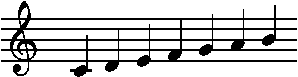
\includegraphics{scores/scale-cropped}
    \end{wrapfigure}
    Waarom do-re-mi-fa-sol-la-si?
    \begin{enumerate}
      \item de structuur van geluid
      \item mooi en lelijk
      \item 7 (of 12) noten
    \end{enumerate}
  \end{block}

  \pause

  \begin{block}{Namiddag}
    Wat maakt geluid muziek?
    \begin{enumerate}
      \item de structuur van geluid analyseren
      \item voorbeelden
      \item verschillen tussen muziekinstrumenten
    \end{enumerate}
  \end{block}
\end{frame}

\begin{frame}
  \frametitle{Vragen staat vrij}
\end{frame}

\section{Wat is geluid?}

\section{Wat zijn boventonen?}
% TODO refer to last part of talk, and afternoon

\section{Hoe maken we verschillende noten?}

\section{Wat klinkt er mooi samen en wat niet?}

\section{Wat is een stemming?}
% TODO: answers the question ``why do we have C D E F G A B''

\section{Wat is het probleem met stemmingen?}

\section{Hoe kunnen we dit oplossen?}

\section{Hoe kan geluid ons bedotten?}
% TODO: end the previous section with a remark hinting at the crappy way we experience sound, ties it in with this last section *and* afternoon
\begin{frame}
  \frametitle{Illusies met geluid}

  % http://tex.stackexchange.com/questions/129274/showcase-of-optical-illusions-made-with-tex-latex-luatex-context
  \centering
  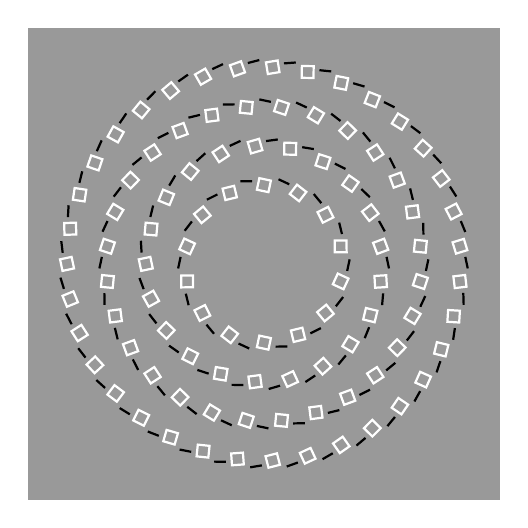
\begin{tikzpicture}[scale = .5]
    \fill[color=black!40!white] (-6,-6) rectangle (6,6);
    \foreach \n/\r/\twist in {70/5/12,56/4/-12,42/3/12,28/2/-12}{
      \foreach \m in {1,3,...,\n}
        \draw [thick,color=white,shift={(360/\n*\m:\r)},rotate=\twist+360/\n*\m] (-.15,-.15) rectangle (.15,.15);
      \foreach \m in {2,4,...,\n}
        \draw [thick,color=black,shift={(360/\n*\m:\r)},rotate=\twist+360/\n*\m] (.15,-.15) rectangle (.15,.15);
      }
  \end{tikzpicture}
\end{frame}

\begin{frame}
  \frametitle{Hoe do-re-mi-fa-sol-la-si ons bedot}

  We weten nu dat
  \begin{center}
    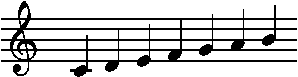
\includegraphics{scores/scale-cropped}
  \end{center}
  overeenkomt met
  \begin{center}
    \begin{tabular}[h]{cccccccc}
      do & re & mi & fa & sol & la & si \\\midrule
      131Hz & 147Hz & 165Hz & 175Hz & 196Hz & 220Hz & 247Hz
    \end{tabular}
  \end{center}
\end{frame}

\begin{frame}
  \frametitle{Een oneindig stijgende toonladder}

  Nu gebruiken we alle twaalf tonen:
  \begin{center}
    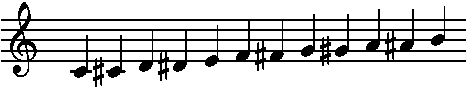
\includegraphics{scores/scale-full-cropped}
  \end{center}
  De frequenties zijn niet zo belangrijk\ldots
\end{frame}

\begin{frame}
  \frametitle{Een toonladder}

  \begin{block}{\twonotes\ audiofragment}
    \texttt{samples/endless.mp3}
  \end{block}
  \pause
  \begin{center}
    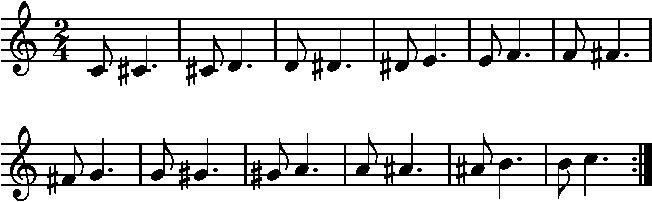
\includegraphics{scores/endless-cropped}
  \end{center}
  \pause
  De toonladder \alert{herhaalt} zich, zonder overgang!
\end{frame}

\begin{frame}
  \frametitle{Wat is er aan de hand?}

  We analyseren het geluid
  % TODO
\end{frame}

\begin{frame}
  \frametitle{Observaties}

  \begin{enumerate}
    \item (alles is een beetje te laag gestemd)
    \item er is geen vastomlijnde grondtoon
    \item de duidelijkste frequentie wordt \alert{zwakker}
    \item de nauwelijks aanwezige laagste frequentie wordt \alert{sterker}
    \item de laatste toon heeft dezelfde samenstelling als de eerste
  \end{enumerate}
\end{frame}

\begin{frame}
  \frametitle{Herhaalde geluidsanalyse}

  We analyseren meerdere kopies van het fragment
  % TODO
\end{frame}

\begin{frame}
  \frametitle{Observaties}

  \begin{enumerate}
    \item we horen de overgang niet, maar \alert{zien} hem wel
    \item exponenti\"eel stijgend
  \end{enumerate}
\end{frame}

\begin{frame}
  \frametitle{Paradox van Shepard}
\end{frame}

\begin{frame}
  \frametitle{Een oneindig dalende glissando}

  Een continue versie van voorgaande paradox
  \begin{block}{\twonotes\ audiofragment}
    \texttt{samples/shepard-risset-glissando.ogg}
  \end{block}
\end{frame}

\begin{frame}
  \frametitle{Paradox van Shepard--Risset}

  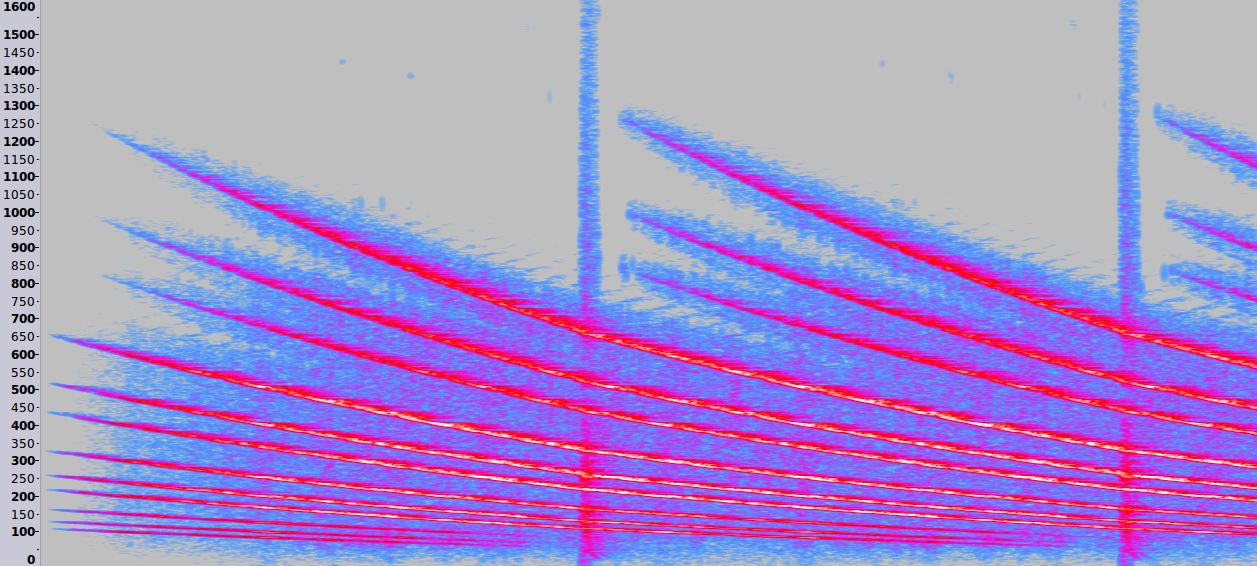
\includegraphics[width=\textwidth]{images/glissando-spectrum.png}
\end{frame}

\begin{frame}
  \frametitle{Een oneindig versnellende beat}
\end{frame}

\begin{frame}
  \frametitle{Paradox van Risset}
\end{frame}
\end{document}

